\documentclass[a4paper, 12pt]{book}
%\documentclass[a4paper, 12pt, draft]{book}  Nalogo preverite tudi z opcijo draft, ki vam bo pokazala, katere vrstice so predolge!
\usepackage[utf8x]{inputenc}   % omogoča uporabo slovenskih črk kodiranih v formatu UTF-8
\usepackage[slovene,english]{babel}    % naloži, med drugim, slovenske delilne vzorce
\usepackage[pdftex]{graphicx}  % omogoča vlaganje slik različnih formatov
\usepackage{fancyhdr}          % poskrbi, na primer, za glave strani
\usepackage{amssymb}           % dodatni simboli
\usepackage{amsmath}           % eqref, npr.
%\usepackage{hyperxmp}
\usepackage[hyphens]{url}  % dodal Solina
\usepackage{comment}       % dodal Solina
\usepackage{spverbatim}       % dodal Jakob
\usepackage[pdftex, colorlinks=true,
						citecolor=black, filecolor=black, 
						linkcolor=black, urlcolor=black,
						pagebackref=false, 
						pdfproducer={LaTeX}, pdfcreator={LaTeX}, hidelinks]{hyperref}
\usepackage{color}       % dodal Solina
\usepackage{soul}       % dodal Solina
%%%%%%%%%%%%%%%%%%%%%%%%%%%%%%%%%%%%%%%%
%	DIPLOMA INFO
%%%%%%%%%%%%%%%%%%%%%%%%%%%%%%%%%%%%%%%%
\newcommand{\ttitle}{Povezovanje gruč Kubernetes}
\newcommand{\ttitleEn}{Connecting Kubernetes clusters}
\newcommand{\tsubject}{\ttitle}
\newcommand{\tsubjectEn}{\ttitleEn}
\newcommand{\tauthor}{Jakob Hostnik}
\newcommand{\tkeywords}{gruča, oblak, Kubernetes, računalniška gruča, povezovanje gruč, mreža gruč, GitOps}
\newcommand{\tkeywordsEn}{cluster, cloud, Kubernetes, computer cluster, connecting clusters, cluster mesh, GitOps}
%%%%%%%%%%%%%%%%%%%%%%%%%%%%%%%%%%%%%%%%
%	HYPERREF SETUP
%%%%%%%%%%%%%%%%%%%%%%%%%%%%%%%%%%%%%%%%
\hypersetup{pdftitle={\ttitle}}
\hypersetup{pdfsubject=\ttitleEn}
\hypersetup{pdfauthor={\tauthor, jakob@hostnik.si}}
\hypersetup{pdfkeywords=\tkeywordsEn}
%%%%%%%%%%%%%%%%%%%%%%%%%%%%%%%%%%%%%%%%
% postavitev strani
%%%%%%%%%%%%%%%%%%%%%%%%%%%%%%%%%%%%%%%%  
\addtolength{\marginparwidth}{-20pt} % robovi za tisk
\addtolength{\oddsidemargin}{40pt}
\addtolength{\evensidemargin}{-40pt}
\renewcommand{\baselinestretch}{1.3} % ustrezen razmik med vrsticami
\setlength{\headheight}{15pt}        % potreben prostor na vrhu
\renewcommand{\chaptermark}[1]%
{\markboth{\MakeUppercase{\thechapter.\ #1}}{}} \renewcommand{\sectionmark}[1]%
{\markright{\MakeUppercase{\thesection.\ #1}}} \renewcommand{\headrulewidth}{0.5pt} \renewcommand{\footrulewidth}{0pt}
\fancyhf{}
\fancyhead[LE,RO]{\sl \thepage} 
%\fancyhead[LO]{\sl \rightmark} \fancyhead[RE]{\sl \leftmark}
\fancyhead[RE]{\sc \tauthor}              % dodal Solina
\fancyhead[LO]{\sc Diplomska naloga}     % dodal Solina
\newcommand{\BibTeX}{{\sc Bib}\TeX}
%%%%%%%%%%%%%%%%%%%%%%%%%%%%%%%%%%%%%%%%
% naslovi
%%%%%%%%%%%%%%%%%%%%%%%%%%%%%%%%%%%%%%%%  
\newcommand{\autfont}{\Large}
\newcommand{\titfont}{\LARGE\bf}
\newcommand{\clearemptydoublepage}{\newpage{\pagestyle{empty}\cleardoublepage}}
\setcounter{tocdepth}{1}	      % globina kazala
%%%%%%%%%%%%%%%%%%%%%%%%%%%%%%%%%%%%%%%%
% konstrukti
%%%%%%%%%%%%%%%%%%%%%%%%%%%%%%%%%%%%%%%%  
\newtheorem{izrek}{Izrek}[chapter]
\newtheorem{trditev}{Trditev}[izrek]
\newenvironment{dokaz}{\emph{Dokaz.}\ }{\hspace{\fill}{$\Box$}}
%%%%%%%%%%%%%%%%%%%%%%%%%%%%%%%%%%%%%%%%%%%%%%%%%%%%%%%%%%%%%%%%%%%%%%%%%%%%%%%
%% PDF-A
%%%%%%%%%%%%%%%%%%%%%%%%%%%%%%%%%%%%%%%%%%%%%%%%%%%%%%%%%%%%%%%%%%%%%%%%%%%%%%%
%%%%%%%%%%%%%%%%%%%%%%%%%%%%%%%%%%%%%%%% 
% define medatata
%%%%%%%%%%%%%%%%%%%%%%%%%%%%%%%%%%%%%%%% 
\def\Title{\ttitle}
\def\Author{\tauthor, jakob@hostnik.si}
\def\Subject{\ttitleEn}
\def\Keywords{\tkeywordsEn}
%%%%%%%%%%%%%%%%%%%%%%%%%%%%%%%%%%%%%%%% 
% \convertDate converts D:20080419103507+02'00' to 2008-04-19T10:35:07+02:00
%%%%%%%%%%%%%%%%%%%%%%%%%%%%%%%%%%%%%%%% 
\def\convertDate{%
    \getYear
}
{\catcode`\D=12
 \gdef\getYear D:#1#2#3#4{\edef\xYear{#1#2#3#4}\getMonth}
}
\def\getMonth#1#2{\edef\xMonth{#1#2}\getDay}
\def\getDay#1#2{\edef\xDay{#1#2}\getHour}
\def\getHour#1#2{\edef\xHour{#1#2}\getMin}
\def\getMin#1#2{\edef\xMin{#1#2}\getSec}
\def\getSec#1#2{\edef\xSec{#1#2}\getTZh}
\def\getTZh +#1#2{\edef\xTZh{#1#2}\getTZm}
\def\getTZm '#1#2'{%
    \edef\xTZm{#1#2}%
    \edef\convDate{\xYear-\xMonth-\xDay T\xHour:\xMin:\xSec+\xTZh:\xTZm}%
}
\expandafter\convertDate\pdfcreationdate 
%%%%%%%%%%%%%%%%%%%%%%%%%%%%%%%%%%%%%%%%
% get pdftex version string
%%%%%%%%%%%%%%%%%%%%%%%%%%%%%%%%%%%%%%%% 
\newcount\countA
\countA=\pdftexversion
\advance \countA by -100
\def\pdftexVersionStr{pdfTeX-1.\the\countA.\pdftexrevision}
%%%%%%%%%%%%%%%%%%%%%%%%%%%%%%%%%%%%%%%%
% XMP data
%%%%%%%%%%%%%%%%%%%%%%%%%%%%%%%%%%%%%%%%  
\usepackage{xmpincl}
\includexmp{pdfa-1b}
%%%%%%%%%%%%%%%%%%%%%%%%%%%%%%%%%%%%%%%%
% pdfInfo
%%%%%%%%%%%%%%%%%%%%%%%%%%%%%%%%%%%%%%%%  
\pdfinfo{%
    /Title    (\ttitle)
    /Author   (\tauthor, jakob@hostnik.si)
    /Subject  (\ttitleEn)
    /Keywords (\tkeywordsEn)
    /ModDate  (\pdfcreationdate)
    /Trapped  /False
}
%%%%%%%%%%%%%%%%%%%%%%%%%%%%%%%%%%%%%%%%%%%%%%%%%%%%%%%%%%%%%%%%%%%%%%%%%%%%%%%
%%%%%%%%%%%%%%%%%%%%%%%%%%%%%%%%%%%%%%%%%%%%%%%%%%%%%%%%%%%%%%%%%%%%%%%%%%%%%%%
\begin{document}
\selectlanguage{slovene}
\frontmatter
\setcounter{page}{1} %
\renewcommand{\thepage}{}       % preprecimo težave s številkami strani v kazalu
\newcommand{\sn}[1]{"`#1"'}                    % dodal Solina (slovenski narekovaji)
%%%%%%%%%%%%%%%%%%%%%%%%%%%%%%%%%%%%%%%%
%naslovnica
 \thispagestyle{empty}%
   \begin{center}
    {\large\sc Univerza v Ljubljani\\%
      Fakulteta za računalništvo in informatiko\\%
      Fakulteta za matematiko in fiziko}%
    \vskip 10em%
    {\autfont \tauthor\par}%
    {\titfont \ttitle \par}%
    {\vskip 3em \textsc{DIPLOMSKO DELO\\[5mm]        
    INTERDISCIPLINARNI UNIVERZITETNI\\ ŠTUDIJSKI PROGRAM PRVE STOPNJE\\ RAČUNALNIŠTVO IN MATEMATIKA}\par}%
    \vfill\null%
    {\large \textsc{Mentor}: izr. prof. dr. Mojca Ciglarič \par}%
   {\large \textsc{Somentor}:  asist. dr. Matjaž Pančur \par}%
    {\vskip 2em \large Ljubljana, 2021 \par}%
\end{center}
% prazna stran
%\clearemptydoublepage      % dodal Solina (izjava o licencah itd. se izpiše na hrbtni strani naslovnice)
%%%%%%%%%%%%%%%%%%%%%%%%%%%%%%%%%%%%%%%%
%copyright stran
\thispagestyle{empty}
\vspace*{8cm}
\noindent
{\sc Copyright}. 
Rezultati diplomske naloge so intelektualna lastnina avtorja in Fakultete za računalništvo in informatiko Univerze v Ljubljani.
Za objavo in koriščenje rezultatov diplomske naloge je potrebno pisno privoljenje avtorja, Fakultete za računalništvo in informatiko ter mentorja.
\begin{center}
\mbox{}\vfill
\emph{Besedilo je oblikovano z urejevalnikom besedil \LaTeX.}
\end{center}
% prazna stran
\clearemptydoublepage
%%%%%%%%%%%%%%%%%%%%%%%%%%%%%%%%%%%%%%%%
% stran 3 med uvodnimi listi
\thispagestyle{empty}
\vspace*{4cm}
\noindent
Fakulteta za računalništvo in informatiko izdaja naslednjo nalogo:
\medskip
\begin{tabbing}
\hspace{32mm}\= \hspace{6cm} \= \kill
Tematika naloge:
\end{tabbing}
TODO
Besedilo teme diplomskega dela študent prepiše iz študijskega informacijskega sistema, kamor ga je vnesel mentor. V nekaj stavkih bo opisal, kaj pričakuje od kandidatovega diplomskega dela. Kaj so cilji, kakšne metode uporabiti, morda bo zapisal tudi ključno literaturo.
\vspace{15mm}
\vspace{2cm}
% prazna stran
\clearemptydoublepage
% zahvala
\thispagestyle{empty}\mbox{}\vfill\null\it%
\noindent
Na tem mestu bi se zahvalil mentorici izr. prof. dr. Mojci Ciglarič za pripravljenost in mentorstvo.
Zahvalil bi se tudi somentorju asist. dr. Matjažu Pančurju za vse nasvete in pomoč pri pisanju diplomske naloge.
Zahvala pa gre tudi moji ženi, staršem, bratom, sestram in prijateljem za podporo in spodbudo pri študiju.
\rm\normalfont
% prazna stran
\clearemptydoublepage
%%%%%%%%%%%%%%%%%%%%%%%%%%%%%%%%%%%%%%%%
% posvetilo, če sama zahvala ne zadošča :-)
\thispagestyle{empty}\mbox{}{\vskip0.20\textheight}\mbox{}\hfill\begin{minipage}{0.55\textwidth}%
Mami Lučki.
\normalfont\end{minipage}
% prazna stran
\clearemptydoublepage
%%%%%%%%%%%%%%%%%%%%%%%%%%%%%%%%%%%%%%%%
% kazalo
\pagestyle{empty}
\def\thepage{}% preprecimo tezave s stevilkami strani v kazalu
\tableofcontents{}
% prazna stran
\clearemptydoublepage
%%%%%%%%%%%%%%%%%%%%%%%%%%%%%%%%%%%%%%%%
% seznam kratic
\chapter*{Seznam uporabljenih kratic}  % spremenil Solina, da predolge vrstice ne gredo preko desnega roba
\noindent\begin{tabular}{p{0.15\textwidth}|p{.375\textwidth}|p{.375\textwidth}}    % po potrebi razširi prvo kolono tabele na račun drugih dveh!
  {\bf kratica} & {\bf angleško}                             & {\bf slovensko} \\ \hline
  {\bf CRD} & custom resource definition & definicija tipov po meri \\
  {\bf DNS} & domain name system & sistem domenskih imen \\
  {\bf IP} & internet protocol & internetni protokol \\
  {\bf HA} & high availability & visoka razpoložljivost \\
  {\bf GA} & general availability & splošna dostopnost \\
  {\bf VPN} & virtual private network & navidezno zasebno omrežje \\
  {\bf TOSCA} & topology and orchestration specification for cloud applications & specifikacija topologije in orkestracije za aplikacije v oblaku \\
  {\bf WAN} & wide area network & prostrano omrežje \\
\end{tabular}
% prazna stran
\clearemptydoublepage
%%%%%%%%%%%%%%%%%%%%%%%%%%%%%%%%%%%%%%%%
% povzetek
\addcontentsline{toc}{chapter}{Povzetek}
\chapter*{Povzetek}
\noindent\textbf{Naslov:} \ttitle
\bigskip

\noindent\textbf{Avtor:} \tauthor
\bigskip
%\noindent\textbf{Povzetek:} 
\noindent 

Ko na naših strežnikih začne zmanjkovati virov obstajata dva standardna načina za povečanje virov v našem sistemu.
Prva možnost je, da nadgradimo naše strežnike, druga pa, da jih kupimo več in jih povežemo v računalniško gručo.
V zadnjih letih se je na slednjem področju zgodil preboj s pojavom sistema Kubernetes.
Sistem je zaradi svoje popularnosti postal de facto standard za upravljanje gruč in orkestracijo kontejnerjev.
A ena sama gruča ni vedno dovolj v primerih, ko imamo težave z dragim prenosom podatkov, preveliko latenco do naših uporabnikov ali pa želimo še bolj povečati stabilnost ali varnost našega sistema.
Pogledali si bomo ozadje povezovanja gruč in kakšne pristope lahko uporabimo za reševanje naših problemov.
Poseben poudarek pa bomo dali tudi sinhronizaciji podatkov, saj je to eden zahtevnejših delov pri upravljanju več računalniških gruč.
Ugotovimo, da nam lahko predstavljene sodobne metode povezovanja gruč zelo olajšajo njihovo upravljanje in preprosto rešijo tudi zahtevnejše probleme sinhronizacije podatkov.

\bigskip
\noindent\textbf{Ključne besede:} \tkeywords.
% prazna stran
\clearemptydoublepage
%%%%%%%%%%%%%%%%%%%%%%%%%%%%%%%%%%%%%%%%
% abstract
\selectlanguage{english}
\addcontentsline{toc}{chapter}{Abstract}
\chapter*{Abstract}
\noindent\textbf{Title:} \ttitleEn
\bigskip

\noindent\textbf{Author:} \tauthor
\bigskip
%\noindent\textbf{Abstract:} 
\noindent 

When we are running low on resources in our computer system, there are two standard solutions for increasing them.
The first solution is to upgrade our servers and the second one is to buy more servers and connect them in a cluster.
There has been a major breakthrough in this field with the release of Kubernetes system in the recent years.
The system became de facto standard for cluster management and container orchestration.
But when we have problems such as expensive data transfer, too much latency to our users, or we want to further increase the stability or security of our system one cluster is not always enough.
We will look at the background of connecting clusters and what approaches we can use to solve our problems.
Furthermore, we will also place special emphasis on data synchronization, as this is one of the more difficult parts of managing multiple computer clusters.
We find that presented modern methods of connecting clusters can greatly facilitate their management and easily solve even more difficult data synchronization problems.

\bigskip
\noindent\textbf{Keywords:} \tkeywordsEn.
\selectlanguage{slovene}
% prazna stran
\clearemptydoublepage
%%%%%%%%%%%%%%%%%%%%%%%%%%%%%%%%%%%%%%%%
\mainmatter
\setcounter{page}{1}
\pagestyle{fancy}
\chapter{Uvod}
\label{uvod}
\section{Motivacija}
Leta 2014 je Google objavil kodo sistema za orkestracijo kontejnerjev Kubernetes~\cite{what-is-Kubernetes}.
Kubernetes  je univerzalni način, ki nam omogoča, da več računalnikov povežemo v gručo, ki deluje kot ena samostojna enota. 
Povezovanje strežnikov v gruče nam vsaj teoretično omogoča visoko razpoložljivost (HA) naših storitev ~\cite{mastering-Kubernetes} in sinhrono delovanje več računalnikov.
V primerih obravnavanih v tem delu pa ni dovolj uporaba ene same gruče, ampak moramo med seboj povezati in upravljati več gruč.
V zadnjem času so razvijalci Kubernetesa začeli bolj celostno reševati ta problem.
Poizkusili so ga rešiti s projektom Federation 1, po njegovi ukinitvi~\cite{kubernetes-federation-evolution}, pa razvijalci Federation 2 oziroma KubeFed trdijo, da bo projekt uspešno prešel iz alfa v beta verzijo~\cite{kubefed-repo}.
\section{Cilj in vsebina naloge}
V tem diplomskem delu bomo obravnavali rešitve problema povezovanja računalniških gruč in primere uporabe, ki izvirajo iz potreb industrije.
Vsakemu primeru bomo poiskali rešitev v Kubernetes okolju z uporabo orodja KubeFed, poudarek pa bomo dali na sinhronizacijo podatkov.
\subsection{Prevelika latenca}
Problem prevelike latence se pojavi v primeru počasnega prenosa podatkov iz naše gruče do uporabnikov.
Ko problem povzroča velika fizična razdalja, ga rešimo s postavitvijo dodatne gruče bližje naših uporabnikov, denimo na njihovo celino.
Če pa postavimo gruče še bližje našim končnim uporabnikom, na primer v njihovo podjetje ali dom, pa govorimo o gručah na robu oblaka.
Zavedati se moramo, da strežniki v gruči zelo veliko komunicirajo, zato je priporočljivo, da so tudi v istem omrežju znotraj istega podatkovnega centra, saj se s tem ponavadi izognemo veliki latenci ~\cite{kube-and-edge}.
\begin{figure}[h]
\begin{center}
  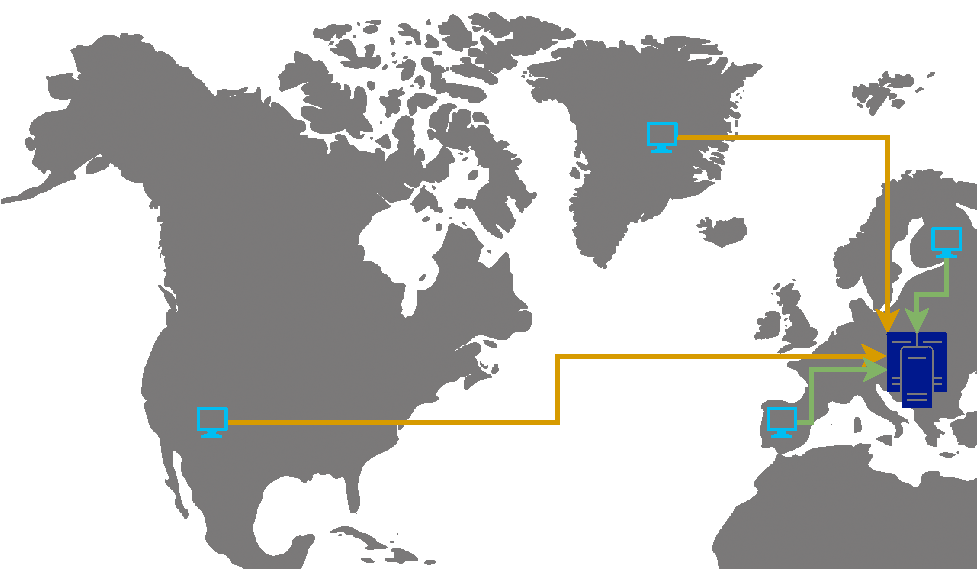
\includegraphics[width=1.0\textwidth]{images/problem-prevelike-latence.pdf}
\end{center}
\caption{Problem prevelike latence.}
\label{problem-prevelike-latence}
\end{figure}
\subsection{Višja razpoložljivost}
Večkrat letno pride do izpada kakšnega večjega podatkovnega centra. 
To se lahko zgodi iz več razlogov najpogosteje pa gre za napake na programski opremi ~\cite{common-outages}.
Če gre v takšnem primeru za oblačnega ponudnika, kjer imamo nameščeno našo gručo, pomeni, da bo hkrati nedosegljiva tudi ta.
V splošnem se problem reši tako, da uporabljamo več gruč in jih namestimo v več različnih podatkovnih centrov.
V primeru izpada enega podatkovnega centra pa naše uporabnike preusmerimo v drug podatkovni center.
\subsection{Potreba po izolaciji aplikacij}
Ko govorimo o izolaciji aplikacije se nanašamo na varnost pri vdoru, ali pa na večjo razpoložljivost.
Uporaba Kubernetesa od nas zahteva izolacijo v kontejnerje.
Prav tako pa nam že Kubernetes sam omogoča izolacijo na posamezne strežnike~\cite{kube-network-policy} ali nastavitev pravil komunikacije v gruči~\cite{kube-pod-to-node}.
Kljub tem postopkom se v Kubernetesu pojavljajo problemi, zaradi katerih postane celotna gruča nedosegljiva, s tem pa vse aplikacije v tej gruči.
Če postavimo del neodvisnih aplikacij v drugo gručo, smo s tem preprečili njihov izpad ob napaki v prvi gruči.
Izolacija pa je pomembna tudi z varnostnega vidika.
Če se napadalec polasti enega samega vozlišča, ima posledično tudi popolno kontrolo nad vsemi drugimi aplikacijami, ki tečejo na tem vozlišču.
Aplikacije lahko pripadajo istemu uporabniku ali pa celo drugim uporabnikom.
Če imamo vsako od naših aplikacij v svoji gruči pa se temu lahko izognemo.
\chapter{Problem povezovanja gruč}
Računalniška gruča je skupina računalnikov, ki zaradi večje zanesljivosti in zmogljivosti skupaj opravlja določene storitve.

Zaradi prevelike latence ali drugih ovir računalnikov ne moremo povezati v eno tesno gručo.
Te računalnike lahko vedno povežemo vsaj v več različnih gruč, četudi to pomeni, da je v nekaterih gručah samo po en strežnik oziroma vozlišče.
Ob prisotnosti povezave pa lahko te gruče med seboj povežeme šibkeje.

Ko govorimo o tesni povezanosti znotraj gruče velja, da ima vsako vozlišče dostop do vsakega, da vsak kontejner lahko komunicira z vsakim, da so vozlišča v istem hitrem notranjem omrežju podatkovnega centra. 
Pričakujemo, da sistem, ki ga uporabljamo za gručenje omogoča razporejanje zaželenih storitev in kontejnerjev med strežniki in v primeru izpada vozlišča to odstrani iz sistema in kontejnerje s tega vozlišča prerazporedi na preostala vozlišča.

Šibka povezanost med gručami pomeni, da je povezava med različnimi gručami počasna, nezanesljiva ali draga.
Zaradi omejitev moramo sprejemati kompromise na podlagi zmožnosti povezave.
Skladno z našimi potrebami se lahko odrečemo komunikaciji med vozlišči v različnih gručah.
Pričakujemo, da vsaka gruča skrbi za svoja vozlišča, ohranja svoje storitve in kontejnerje v delovanju.
Naloge sistemov za povezovanje gruč pa so: omogočanje centralnega nadzora nad storitvami v gručah, prerazporejanje teh storitev med gručami, dinamično odkrivanje drugih gruč in njihovih storitev, izločanje nedosegljivih gruč, povezljivost med vsemi vozlišči in kontejnerji, četudi so vozlišča v različnih omrežjih.

\begin{figure}[h]
\begin{center}
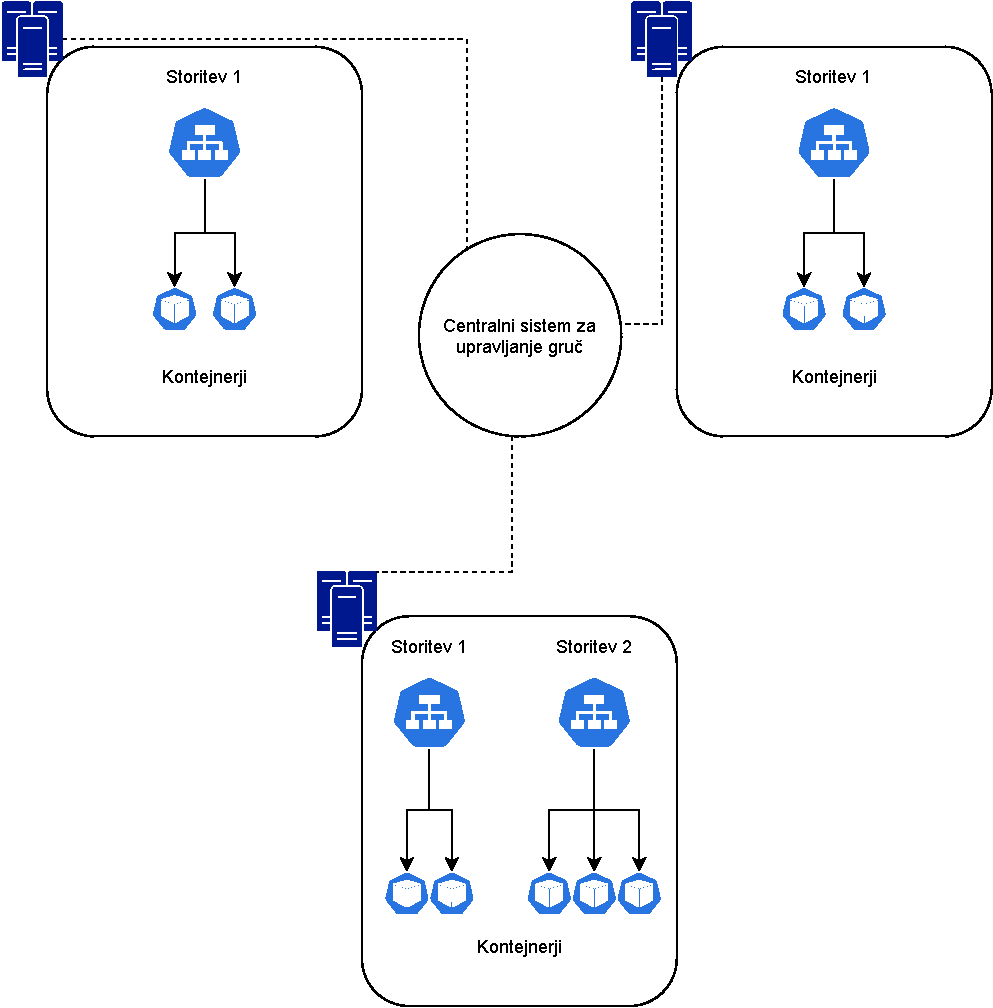
\includegraphics[width=1.0\textwidth]{images/primer-povezanih-gruc.pdf}
\end{center}
\caption{Primer povezanih več gruč.}
\label{problem-povezanih-gruc}
\end{figure}

\chapter{Kubernetes}
\label{Kubernetes}
Kubernetes definira javno dostopen vmesnik REST.
Trenutno obstaja že več kot 70 distribucij~\cite{cncf} Kubernetesa.
\section{Zgodovina~\cite{mastering-kubernetes}}
Leta 2014 je Google objavil in odprl kodo projekta Kubernetes~\cite{what-is-Kubernetes}.
Gre za program, ki je bil ustvarjen z namenom, da poenostavi upravljanje kontejnerjev in večjih računalniških gruč v produkcijskih okoljih.
A to vseeno niso pravi začetki Kubernetesa.
Začelo se je leta 2003, ko je Google začel z razvojem sistema za upravljanje njihovih notranjih gruč Borg.
Kasneje leta 2013 je Google predstavil sistem Omega.
Leta 2014 pa je Google objavil odprtokodni projekt Kubernetes. 
Projekt je bil zasnovan na podlagi dobrih praks upravljanja s kontejnerji, ki so se jih pri Googlu naučili skozi leta.
Kasneje je upravljanje nad projektom prevzela organizacija Cloud Native Computing Fundation.
\section{Osnovni pojmi}
Kubernetesov vmesnik REST nam omogoča, da v Kubernetes shranjujemo najrazličnejše tipe objektov.
Takšne, ki so del standardnega Kubernetesovega API-ja ali pa smo jih definirali sami (CRD).
Najpogostejši tipi objektov, ki se pojavijo v Kubernetesu so pod, service, deployment, statefulset in objekti za delo z diski.
\begin{figure}[h]
\begin{center}
\includegraphics[width=1.0\textwidth]{images/Kubernetes-simple-schema.pdf}
\end{center}
\caption{Primer delovanja Kubernetes objektov.}
\label{problem-povezanih-clustrov}
\end{figure}
\subsection{Pod~\cite{pod}}
Objekt pod je najmanjša enota v Kubernetesu, ki lahko teče v gruči.
Sestavljen je iz enega ali več kontejnerjev, ki si delijo diske in omrežni vmesnik.
To pomeni, da imajo skupen IP in se obnašajo podobno kot izolirani procesi na istem računalniku.
\subsection{Service~\cite{service}}
Objekt service označuje vse pode ene mikrostoritve.
Kubernetes iz objekta v notranjem DNS ustvari domeno za mikrostoritev in dinamično razvršča promet med našimi podi.
Service objekte uporabljamo tako, da namesto pošiljanja zahtevkov direktno na IP naslov Poda, delamo klice na ustvarjeno domensko ime storitve na primer \spverb|curl ime-storitve|.
Takšen zahtevek potem dobi en izmed označenih podov v objektu service.
\subsection{Deployment~\cite{deployment}}
Deployment je objekt, ki mu podamo število željenih objektov pod in predlogo za njihovo izdelavo.
Potem pa notranje storitve Kubernetesa zagotavljajo, da bo obstajalo toliko takšnih objektov tipa pod kot smo navedli v deploymentu.
Takšno stanje se poizkuša ohranjati tudi ob raznih težavah in izpadih vozlišč.
\subsection{StatefulSet~\cite{statefulset}}
Objekt zelo podoben deploymentu, le da statefulset vsakemu podu dodeli unikatno številko. 
Pod, ki se ustvari s to številko ohranja diske, mrežni vmesnik, IP naslov in domensko ime.
Pomembna razlika med objektoma deployment in statefulset pa je tudi v polju \spverb|volumeClaimTemplate|.
Statefulset omogoča vsakemu podu, da si ustvari in uporablja svoj disk.
Uporablja pa se za podatkovne baze in podobne storitve, ki morajo ohranjati stanja.
\chapter{Pregled področja in literature}
V tem poglavju si bomo pogledali nekaj ključnih del in literature na področju povezovanja gruč Kubernetes.
V delih je pogosto za federacijo izbran sistem Federation 1 ali Federation 2 zaradi tesne povezanosti s sistemom Kubernetes~\cite{tosca-fed}~\cite{dyn-place}~\cite{kube-and-edge}.

V članku \cite{tosca-fed} se avtorji lotijo povezovanja gruč pri različnih oblačnih ponudnikih.
Pri tem pozornost namenijo tudi avotmatskemu horizontalnemu skaliranju aplikacij.
Za uporabo in postavitev pri več oblačnih ponudnikih so uporabili standard TOSCA, ki jim omogoča enoten deklarativni zapis njihove strukture v različnih oblakih.
V svoji študiji so uporabili sistem Cloudify, ki pa jim z dodatkom za Kubernetes omogoča tudi enoten način namestitve Kubernetesa.
Svoje gruče so še povezali v federacijo s sistemom Federation. 
Iz članka pa ni povsem razvidno ali so uporablili prvo ali drugo iteracijo sistema Federation.
V testne namene pa so v federacijo namestili še strežnik spletne igre in pokazali uspešnost avtomatskega horizontalnega skaliranja.

Lorenzo Martino je v svoji magistrski nalogi ~\cite{dyn-place} v uvodu pojasnil pomembnost pristopa mikrostoritev pri razvoju aplikacij in pokazal prednosti uporabe Kubernetesa v oblaku.
Kot glavno prednost je izpostavil neodvisnost od platforme in možnost uporabe sistema Kubernetes v oblaku ali pa v svojem podatkovnem centru.
Omenil je tudi hibridne rešitve, ki pa zahtevajo povezovanje in upravljanje večih gruč.

V nadaljevanju je podanih nekaj predlogov za uporabo več gruč Kubernetes, kot so: izolacija med produkcijskim in testnim okoljem, težave z latenco zaradi prevelikih fizičnih razdalj, povečevanje razpoložljivosti aplikacije, uporaba dodatne gruče v oblaku zaradi lažjega avtomaskega skaliranja vozlišč, omejitve lokacije obdelovanja podatkov.
V delu je predlaganih tudi nekaj programov za upravljanje gruč, v rešitvi svojega problema pa je uporabil sistem KubeFed.
Avtor omeni, da je pri svojem delu reševal problem v podjetju, ki se ukvarja s civilnimi in vojaškimi aeronavtičnimi sistemi.
Ključna zahteva v podjetju pa je bila obdelava podatkov v lokalnih gručah.
Nadaljevanje dela je vezano na reševanje konkretnega problema podjetja.
Sinhronizaciji podatkov je v delu namenjena posebna pozornost, saj imajo v podjetju označene podatke, ki se ne smejo obdelovati v oblaku in podatke, ki se lahko.
KubeFed je še v razvojni fazi alfa, kar pa je predstavljalo oviro za podjetje.
Tako avtor poleg rešitve s KubeFed pripravi še svojo rešitev, kjer implementira samo potrebne funkcionalnosti.

Vir ~\cite{kube-and-edge} pa se posveti področju upravljanja aplikacij na robu oblaka, kjer zaradi večjega števila gruč centralno upravljanje pride še bolj do izraza.
V poročilu je postavljena gruča Kubernetes v prostrano omrežje (WAN).
Avtorji so primerjali delovanje ene gruče preko prostranega omrežja z delovanjem iste gruče preko lokalnega omrežja.
Izpostavijo pomembnost previdnosti pri takšnem pristopu v gručah na robu oblaka, saj lahko pride do nepredvidljivih rezultatov.
V poročilu je predstavljen tudi odprtokodni sistem KubeEdge.
Projekt je namenjen razširitvi aplikacij v kontejnerjih na vozlišča na robu oblaka~\cite{kubeedge}.
Avtorji izpostavijo, da imata tako pristop z eno gručo v omrežju WAN kot pristop z KubeEdge pomembno omejitev, saj imajo vozlišča še vedno premalo avtonomnosti v primeru izpada iz omrežja.
Izpostavljeno je, da te slabosti rešimo s federacijo in sistemom KubeFed, ki je v nadaljevanju podrobneje opisan.
Če je vsako vozlišče v svoji gruči potem je vozlišče v primeru izpada omrežja še vedno avtonomno in omogoča lokalno upravljanje.

\chapter{Povezovanje gruč Kubernetes}
Ko postavimo več različnih gruč imamo vedno možnost, da upravljamo vsako posebej.
A takšen pristop je neučinkovit, če imamo takšnih gruč res veliko~\cite{difference-multi-cluster}.
Osnovna lastnost sistema za upravljanje več gruč Kubernetes, je možnost prenašanja Kubernetesovih objektov med gručami.
Tako lahko objekt definiramo samo enkrat in bo naš sistem ta objekt ustvaril v izbranih gručah.
Odvisno od naših potreb pa lahko uporabimo sistem, ki omogoča tudi dinamično odkrivanje storitev z enako definicijo v različnih gručah, komunikacijo med storitvami v različnih gručah, dinamično odkrivanje podov med gručami in komunikacijo med podi v različnih gručah.
Te funkcionalnosti znotraj ene gruče nudi že Kubernetes sam.
Je pa seveda odvisno od našega primera, katere funkcionalnosti želimo uporabiti in kako kompleksno postavitev potrebujemo.
V nadaljevanju si bomo ogledali različne sisteme za povezovanje gruč Kubernetes, njihove glavne prednosti in značilnosti.
\section{ArgoCD in drugi sistemi GitOps}
\subsection{Sinhronizacija objektov z uporabo sistemov GitOps}
Osnovna ideja pristopa GitOps je, da imamo našo strukturo aplikacij v gruči Kubernetes napisano v repozitoriju Git in potem je kontroler GitOps tisti, ki iz teh definicij postavi strukturo gruče.
Takšen pristop se je v zadnjih letih zelo razširil in ArgoCD navaja več kot 100 podjetji, ki pri razvoju svojih spletnih aplikacij uporabljajo pristop GitOps~\cite{argocd-user-list}.

Če uporabljamo kakšnega od sistemov GitOps, lahko potem iz enakega repozitorija postavimo več gruč.
V osnovi takšen pristop pomeni, da bomo imeli na voljo samo sinhronizacijo infrastrukture in nam takšen pristop ne omogoča naprednih funkcionalnosti kot so komunikacija med podi v različnih gručah ali pa odkrivanje storitev ali podov.
V nadaljevanju si bomo izbrali sistem ArgoCD in si pogledali, kako bi si postavili zgoraj opisano infrastrukturo.
\subsection{Sinhronizacija objektov z ArgoCD}
ArgoCD podpira več različnih formatov konfiguracije gruče~\cite{argocd-docs}.
Uporabimo lahko YAML format datoteke z definicijami objektov, ki jih želimo namestiti v vsako gručo.
Za nameščanje te konfiguracije v več kot eno gručo imamo na voljo dva pristopa.
Prvi način je, da v vsako gručo namestimo ArgoCD in uporabimo enak repozitorij Git v vseh.
ArgoCD pa nam omogoča tudi pošiljanje konfiguracije v oddaljene gruče~\cite{declarative-setup}.
To pomeni, da imamo lahko kontroler ArgoCD nameščen samo v eni gruči.

Če ne želimo, da imajo vse gruče popolnoma enako infrastrukturo in nameravamo prilagoditi konfiguracijo posameznege gruče.
V tem primeru bi uporabili format zapisa konfiguracije, ki podpira predloge.
ArgoCD nam ponuja možnost, da ročno določimo spremenljivke predlogam.
Tako lahko uporabimo na primer predloge HELM in ArgoCD nam bo omogočil, da vsaki gruči izberemo svojo datoteko s spremenljivkami.
Glede na preprostost delovanja takšnega sistema se moramo zavedati, da od njega ne moremo pričakovati nikakršnih naprednih funkcionalnosti kot sta dinamično odkrivanje storitev ali komunikacija podov med gručami.
Takšen sistem nam omogoča samo sinhronizacijo infrastrukture.

\begin{figure}[h]
\begin{center}
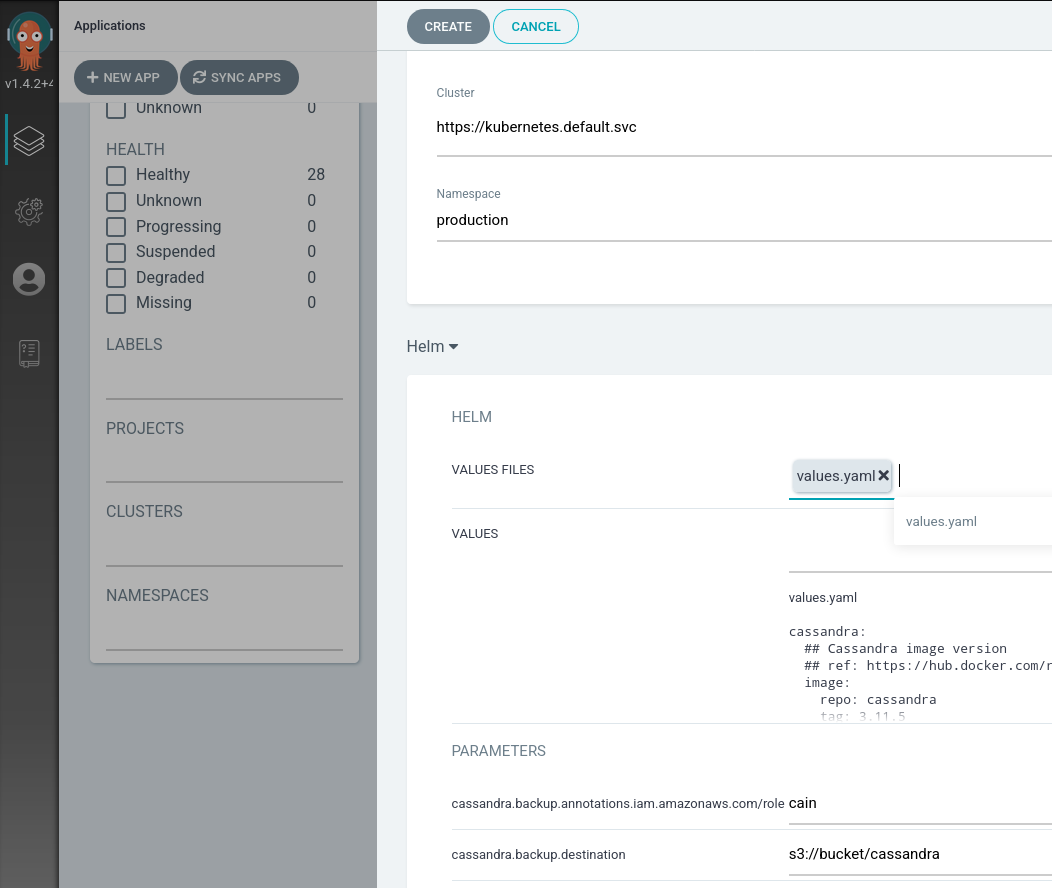
\includegraphics[width=1.0\textwidth]{images/primer-uporabe-helm-predloge-argo-cd.png}
\end{center}
\caption{Primer uporabe predloge HELM v ArgoCD.}
\label{primer-uporabe-helm-predloge-argo-cd}
\end{figure}


\section{KubeFed}
9. 1. 2018 je bil po ukinjenem projektu Kubernetes Federation V1 ustvarjen Kubernetes Federation V2 imenovan tudi KubeFed~\cite{kubernetes-federation-evolution}.
Cilj obeh projektov je bil poenostavljeno upravljanje več gruč in razporejanje Kubernetes objektov.
V projektu Federation V1 je bil ubran pristop, ki je skupino gruč ali federacijo uporabniku predstavil kar kot novo gručo Kubernetes~\cite{setup-cluster-federation-kubefed-v1}.
Uporabljal je svoj API in kontroler API, ki pa je bil združljiv s Kubernetesovim, kar pa je omogočalo tudi uporabo orodja kubectl~\cite{cluster-federation-in-Kubernetes-1.5}.
Objekti, ki jih je federacija podpirala so bili kompatibilni s standardnimi Kubernetes objekti~\cite{federated-cluster-kubefed-v1}.
Objekte, ki so bili poslani kontrolerju federacije, je potem Federation V1 ustvaril tudi v pripadajočih gručah.
Pristop zaradi mnogih pomanjkljivosti in pomankanja možnosti naprednejših konfiguracij ni uspel pridobiti statusa GA.
GA faza v Kubernetesu pomeni, da se uporabniki lahko zanašajo na projekt, ga uporabljajo in se bo vsaj do neke mere ohranjala združljivost za nazaj.
  Pred dosegom te stopnje naj bi se projekt uporabljalo samo v testne namene.

Tako se je kasneje razvil projekt Federation V2~\cite{kubernetes-federation-evolution}.
Glavna razlika s prvo verzijo z uporabniškega stališča je v tem, da za federacijo ne poizkuša imitirati Kubernetesovega API-ja, ampak uporablja obstoječi Kubernetesov API. 
Federation V2 samo predstavi nove objekte, ki pa so razširitev standardnih, kot na primer federateddeployment~\cite{kubefed-userguide}.
Federated objekte je treba najprej vklopiti z ukazom \spverb|kubefedctl enable|.
\begin{verbatim}
kubefedctl enable deployment
\end{verbatim}
Orodje kubefedctl si moramo namestiti na naš računalnik.
Takšen Federated objekt vsebuje tri glavne lastnosti: definicija predloge primarnega objekta, postavitev v gruče in prepis lastnosti originalnega objekta za posamezne gruče.
Takšen pristop je zelo široko zastavljen in omogoča tudi federacijo CRD objektov.
\begin{verbatim}
apiVersion: types.kubefed.io/v1beta1
kind: FederatedDeployment
spec:
  placement:
    clusterSelector:
      # izbira gruč
      matchLabels: {}
      ... 
  template:
    # specifikacije deployment objekta
    spec:
    ... 
  overrides:
    # prepis konfiguracije za posamezne gruče
    - clusterName: gruca-1
      clusterOverrides:
          # nastavi polje replicas na vrednost 5
        - path: "/spec/replicas"
          value: 3
  ... 
\end{verbatim}
Federation V2 podpira poleg sinhronizacije infrastrukture tudi odkrivanje storitev v drugih gručah prek DNS zapisov~\cite{kubefed-userguide}.
Omenja pa se možnost odstranitve te funkcionalnosti~\cite{remove-service-discovery}, ki je že sedaj privzeto izklopljena.
Preden pa uporabimo KubeFed pa se moramo zavedati, da je projekt v času pisanja diplomske naloge še vedno v razvojni fazi alfa in lahko mine še nekaj časa preden doseže status GA, če slučajno ne bo šel po stopinjah svojega predhodnika.
\section{Cilium}
Cilium je odprtokodni program, ki nam omogoča napredne varnostne in omrežne nastavitve v naši gruči~\cite{cilium-intro}.
Program na tretji in četrti omrežni plasti zagotavlja osnovne principe varnosti in zaščite, kot na primer zapiranje portov in omejevanje komunikacije.
Poleg tega pa Cilium zagotavlja tudi naprednejšo varnost na sedmi omrežni plasti, saj nam omogoča omejevanje in filtriranje HTTP zahtevkov in podobne varnostne funkcionalnosti na popularnih protokolih aplikacijskega nivoja~\cite{cilium-intro}.

Ker Cilium implementira precejšni del mreženja in povezovanja v Kubernetesu, pa nam s tem lahko ponudi tudi nekaj zelo naprednih možnosti, ko med seboj povezujem več različnih gruč Kubernetes.
Tako nam kot ključno prednost Cilium omogoča tudi komunikacijo med podi v različnih gručah~\cite{cilium-cluster-mesh} in uporabo globalnih objektov service, ki razporejajo promet med različnimi gručami.
Takšne objekte definiramo z anotacijo \spverb|io.cilium/ global-service|~\cite{setup-cilium-cluster-mesh}.
Omogoča nam tudi omejevanje povezovanja med gru\-ča\-mi z njihovim objektom \spverb|CiliumNetworkPolicy|~\cite{setup-cilium-cluster-mesh}.
Ko postavljamo mre\-žo gruč, pa se moramo še vedno zavedati, da Cilium ne rešuje problema, če so naše gruče skrite v različnih zasbenih omrežjih.
Ključno pri uporabi Ciliuma za povezovanje gruč je, da so vsa naša vozlišča dosegljiva med seboj.
A četudi so naše gruče v med seboj nedosegljivih zasebnih omrežjih, pa je problem rešljiv z uporabo sistema VPN, ki nam omogoča, da vsa vozlišča povežemo v eno navidezno omrežje~\cite{setup-cilium-cluster-mesh}.

Kljub naprednim funkcijam, ki nam jih Cilium ponuja, pa se moramo zavedati, da se Cilim ukvarja samo s povezovanjem gruč na omrežnem nivoju.
Ne omogoča enotnega upravljanja in sinhroniziranja objektov med gručami zato moramo objekte sinhronizirati sami.
Ampak zaradi dovolj široke zasnove Kubernetesovega vmesnika so rešitve med seboj kompatibilne.
Torej lahko uporabimo napredno mreženje Ciliuma in objekte sinhroniziramo s pristopom KubeFed ali GitOps.
\chapter{Priprava sistema gruč za testiranje}
\section{Raspberry PI 4}
Za namene testiranja različnih načinov povezovanja gruč Kubernetes moramo najprej postaviti nekaj gruč.
Zaradi preprostosti in nizke cene, predvsem pa ker se koncepti zaradi tega ne spremenijo, bomo za naša Kubernetes vozlišča uporabili Raspberry PI 4.
Na višjem nivoju pa gre še vedno za gručo Kubernetes in je delo zelo podobno, če uporabimo nekaj 1000 vozlišč v gruči v oblaku ali pa lokalno gručo z enim vozliščem.
Raspberry PI 4 je majhen (85x56x20mm) in manj zmogljiv računalnik na eni sami plošči~\cite{rpi-tech-spec}.
Ključni prednosti takšnih računalnikov pa sta velikost in cena.
Na vsak Raspberry PI se bo namestila gruča Kubernetes z enim samim vozliščem.
Fizična postavitev gruč je prikazana na sliki \ref{rpi-gruce}.
Takšna postavitev pa je lahko tudi primer gruče na robu oblaka, kar je bolj podrobno opisano v poglavju \ref{edge-clusters}.
\begin{figure}[h]
\begin{center}
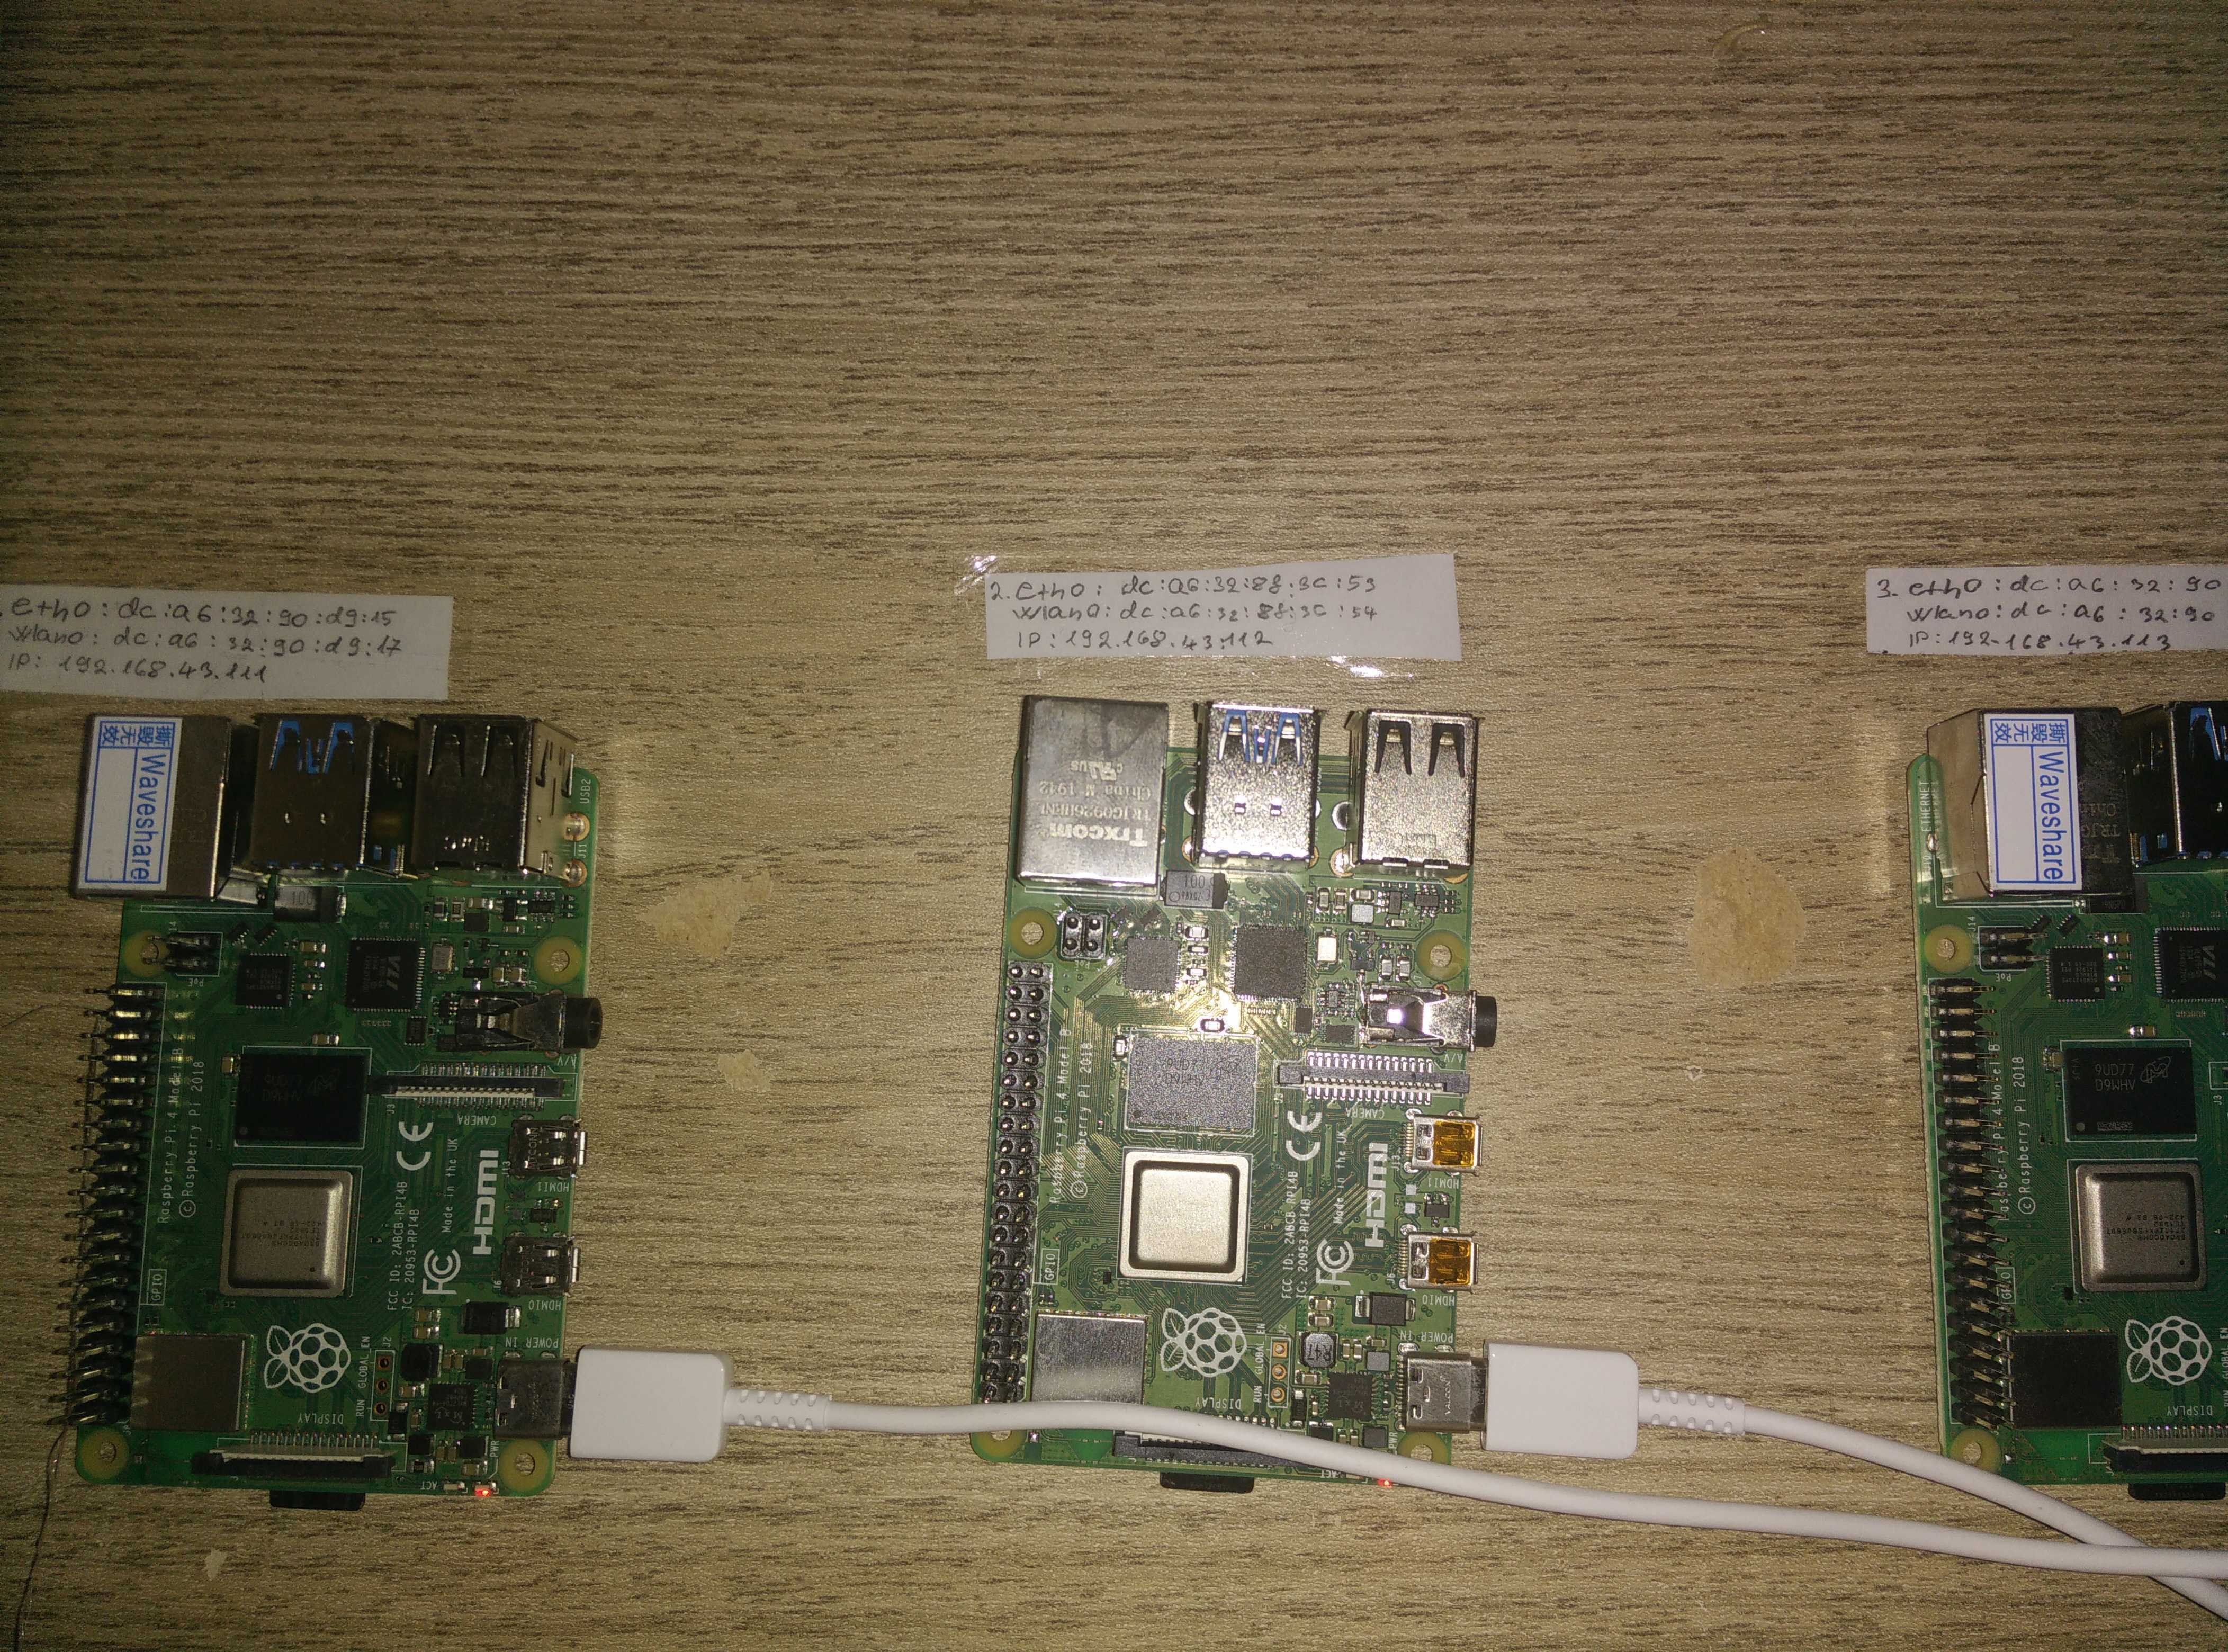
\includegraphics[width=1.0\textwidth]{images/postavitev-raspberry.jpg}
\end{center}
\caption{Postavitev gruč Raspberry PI.}
\label{rpi-gruce}
\end{figure}
\section{K3S in K3OS}
Obstaja več implementacij Kubernetesa in mi bomo uporabili z viri varčno odprtokodno implementacijo K3S od podjetja Rancher~\cite{k3s-info}.
Hkrati so v podjetju Rancher pripravili distribucijo operacijskega sistema Linux K3OS~\cite{k3os-git}.
Gre za minimalen operacijski sistem s prednameščenim sistemom K3S.
Te\-ža\-va se pojavi, ker še ni pripravljene uradne verzije operacijskega sistema za ploščice Raspberry PI.
A k sreči se je v ta namen začel odprtokodni projekt \sn{PiCl k3os image generator}, ki nam iz slik operacijskih sistemov K3OS in Raspberry OS in konfiguracijskih datotek zgradi novo sliko operacijskega sistema za naš Raspberry PI ~\cite{k3os-rpi-image-generator}.
Konfiguracijske datoteke, ki jih moramo priložiti so standardne YAML datoteke, ki jih podpira sistem K3OS.
Vanje zapišemo nastavitve kot so SSH javni ključi za dostop, podatki od WiFi omrežja na katerega se povezujemo, geslo, žeton za povezavo s gručo Kubernetes in način v katerem želimo zagnati K3S na sistemu~\cite{k3os-git}.
\begin{figure}[h]
  \begin{verbatim}
ssh_authorized_keys:
- ssh-rsa ...
hostname: gruca-1
k3os:
  ntp_servers:
  - ...
  password: ...
  token: ...
  dns_nameservers:
  - ... 
  wifi:
  - name: ...
    passphrase: ...
  k3s_args:
  - server
\end{verbatim}
\end{figure}
V našem primeru smo vse K3S programe zagnali v strežniškem načinu (server) in nobenega v načinu delovnega vozlišča, saj želimo, da vsak Raspberry PI predstavlja svojo gručo.
\section{Demonstracijska spletna aplikacija}
Za potrebe testiranja je bilo potrebno naredili novo testno mikrostoritev.
Ker se v tem diplomskem delu želimo osredotočiti na industrijske probleme, mora ta aplikacija omogočati tudi shranjevanje podatkov v podatkovno bazo.

Koda, ki je javno objavljena v repozitoriju Git~\cite{git-stateful-rest-sample}, je napisana v programskem jeziku Go.
Iz kode je bil generiran kontejner, ki je objavljen v javnem Docker repozitoriju~\cite{docker-stateful-rest-sample}.
Ob tem velja opozoriti, da Raspberry PI uporablja ARM arhitekturo procesorja, kar je zahtevalo dodatno pozornost.

Aplikacija deluje preprosto.
Na mrežnih vratih podanih s spremenljivko okolja izpostavi vmesnik REST z dvema preprostima HTTP klicema.
\spverb|GET| klic na pot \spverb|/users| nam bo vrnil seznam vseh uporabnikov, ki so zapisani v tabeli v podatkovni bazi, s klicem \spverb|POST| na isto pot pa poskrbimo, da se podatki uporabnika iz našega zahtevka shranijo v tabelo v podatkovni bazi.
\begin{verbatim}
# ukaz za dodajanje uporabnika
curl -X POST localhost/users \
  --data '{"name": "John", "lastname": "Doe"}'
# ukaz za prikaz vseh uporabnikov
curl localhost/users
\end{verbatim}

Za shranjevanje podatkov bomo uporabili 2 različni SQL bazi podatkov.
Postgres, ki je preprosta za lokalni razvoj, a ne omogoča napredne sinhronizacije podatkov med strežniki in CrateDB, ki je bil zasnovan kot SQL baza na več vozliščih in nam omogoča napredne sinhronizacije tudi med različnimi strežniki in gručami.
K sreči pa CrateDB implementira vmesnik PostgreSQL in nam kode za prehod med bazami ni potrebno spreminjati~\cite{cratedb}.
\section{Namestitev KubeFed}
Kot ena izmed ključnih komponent složnega delovanja več gruč je njihovo upravljanje.
V te namene bomo uporabili program KubeFed, ki ga moramo namestiti na eno izmed gruč, ki jih želimo povezati skupaj.
Ker je izdelek še v razvoju in še ni prišel iz alfa faze, še ni objavljene verzije programa za procesorje ARM.
Zato je bilo iz kode KubeFed potrebno zgraditi novo sliko kontejnerja, ki je javno objavljena~\cite{docker-kubefed}.
Potem pa smo uporabili originalno HELM predlogo, kjer smo samo zamenjali originalno sliko kontejnerja z našo.
Za delo s KubeKed pa moramo na svoj računalnik namestiti še orodje kubefedcli.
Z uporabo ukaza \spverb|kubefedctl join| povežemo vse tri gruče v kubefed sistem.
\begin{verbatim}
kubefedctl join gruca-1
kubefedctl join gruca-2
kubefedctl join gruca-3
\end{verbatim}
S tem smo uspešno povezali več gruč Kubernetes v sistem KubeFed.
Seznam vseh povezanih gruč pa lahko preverimo tako, da izpišemo seznam objektov tipa kubefedclusters. 
V našem primeru imamo povezane tri gruče, kar se vidi iz sledečega izpisa.
\begin{verbatim}
kubectl get kubefedclusters

NAME        AGE   READY
gruca-1     1d    True
gruca-2     1d    True
gruca-3     1d    True
\end{verbatim}
Sedaj lahko z uporabo ukazov \spverb|kubefedctl enable| in \spverb|kubefedctl federate| naše objekte dodajamo v vse gruče hkrati.
Več o tem je napisano v poglavjih, kjer ukaze tudi uporabljamo.

\chapter{Povezovanje med podatkovnimi centri}
\label{povezovanje-med-centri}
\section{Problem velike latence}
Za primer vzemimo preprosto spletno aplikacijo, ki mora hraniti stanje in jo namestimo v eno gručo Kubernetes.
Če našo aplikacijo ponudimo vsem uporabnikom na globalnem trgu se nam bo pojavil problem velike latence.
To pomeni, da bo naša aplikacija za uporabnike, ki so bolj oddaljeni od naše gruče delovala počasneje oziroma se bodo podatki do uporabnika prenašali dalj časa.

Takšen problem v splošnem rešimo tako, da našo aplikacijo postavimo še v dodatno gručo bližje uporabniku. 
Če pa moramo podatke med gručami še sinhronizirali pa to zahteva dodaten trud.
V našem primeru bomo uporabili podatkovno bazo CrateDB~\cite{cratedb}, novejšo alternativo standardnim SQL podatkovnim bazam.
CrateDB ima v primerjavi s tradicionalnimi podatkovnimi bazami boljšo podporo za sinhronizacijo podatkov med vozlišči.
Poleg vsega pa nam za uporabo podatkovne baze CrateDB ni potrebno konceptualno spreminjati naše aplikacije, saj podpira vmesnik podatkovne baze PostgreSQL.
\section{Povečanje razpoložljivosti aplikacije}
Če je čim višja razpoložljivost za našo aplikacijo kritičnega pomena in smo že poskrbeli za visoko razpoložljivost (HA) aplikacije v naši gruči, še vedno lahko pride do situacije, ko iz omrežja izpade cel podatkovni center.
Spomnimo se, da Kubernetes najbolj učinkovito deluje, če naša vozlišča uporabljajo hitro notranje omrežje podatkovnega centra.
V primeru napake v podatkovnem centru ali hujših vremenskih pogojev pomeni, da je nedosegljiv cel podatkovni center in s tem gruča v njem.
Če uporabljamo strežnike v oblaku, pa gremo lahko še korak dlje z zagotavljanjem razpoložljivosti.
Če nam ni dovolj niti to, da uporabimo različne razpoložljivostne cone in podatkovne centre oblačnih ponudnikov, lahko postavimo naše gruče pri več različnih ponudnikih.
Takšen pristop je opisan v članku~\cite{tosca-fed}, omogoča pa ga predvsem neodvisnost Kubernetesa od platform.
\section{Povezovanje med podatkovnimi centri}
Rešitev za oba omenjena problema je enaka.
Postaviti moramo gruče v več različnih podatkovnih centrih in jih nastaviti, da bodo delovale usklajeno.
Odvisno od problema bodo te podatkovni centri bližje uporabniku ali pa v lasti različnih oblačnih ponudnikov.
A princip ostaja enak.
\section{Razporeditev uporabnikov po gručah}
Ko imamo na vsaki gruči javno izpostavljen Kubernetesov service objekt in postavljene primerne ingress objekte, moramo še vedno uporabnike preusmeriti na njim najbližjo gručo.
Uporabnike lahko mi usmerimo avtomatsko z DNS zapisi, ki omogočajo usmerjanje na podlagi geolokacije.
Lahko uporabimo in namestimo zunanji DNS skozi Kubernetes ali pa to opravimo kar mimo Kubernetesa.
V naših lokalnih testnih gručah bomo ta korak preskočili in jih ne bomo usmerjali preko javnih DNS strežnikov, saj v lokalnem okolju to ni smiselno.
\begin{figure}[h]
\begin{center}
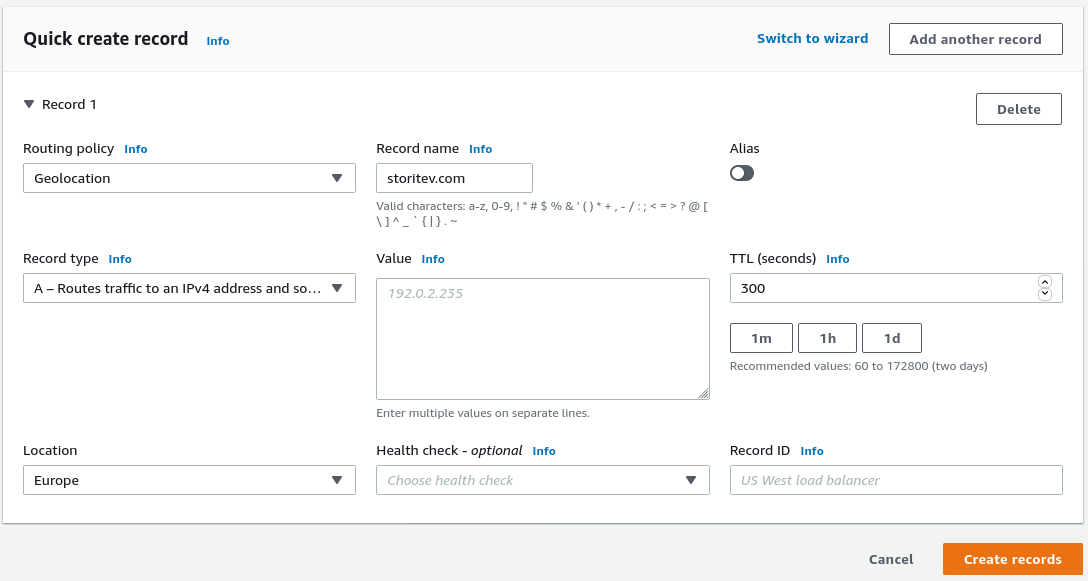
\includegraphics[width=1.0\textwidth]{images/geolokacijski-dns.png}
\end{center}
\caption{Ustvarjanje geolokacijskega DNS zapisa v storitvi ROUTE53.}
\label{primer-ustvarjanje-geolokacijskega-zapisa}
\end{figure}

Naslednja možnost pa je rešitev, ki se jo poslužujejo nekatere internetne računalniške igre (npr. Among US), da so naši strežniki popolnoma ločeni in se vsak uporabnik sam odloči na kateri gruči ali strežniku želi igrati.
V takšnih primerih se lahko tudi izognemo problemu sinhronizacije podatkov med strežniki, kar zelo poenostavi upravljanje naših gruč.
\section{Definicija infrastrukture za naš primer}
V našem primeru spletne aplikacije bomo imeli v vsaki gruči eno postavitev aplikacije \sn{Stateful rest sample} z deployment objektom. 
Da aplikacijo izpostavimo izven gruče, pa bomo uporabili objekt service.
Aplikacija bo za shranjevanje uporabljala podatkovno bazo CrateDB, ki bo postavljena z objektom statefulset, diskom na lokalni SD kartici, in dvema objektoma service.
Prvi objekt service je zunanji in se bo uporabljal za dostop do baze, drugi pa je notranji in ga bomo uporabljali za prepoznavo ostalih primerkov CrateDB v gruči.
\begin{figure}[h]
\begin{center}
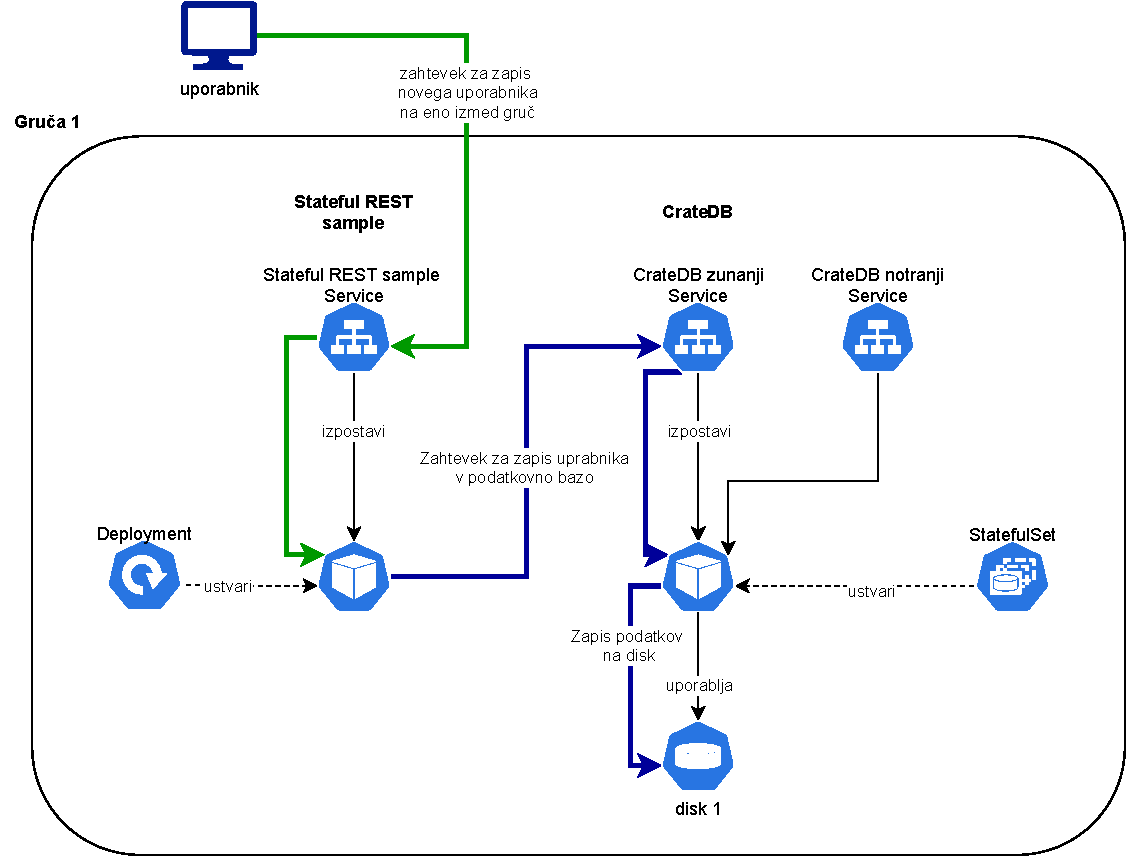
\includegraphics[width=1.0\textwidth]{images/infrastructure-example.pdf}
\end{center}
\caption{Infrastruktura vsake gruče v primeru demonstracijske aplikacije}
\label{infrastructure-example}
\end{figure}
Vsa konfiguracija je javno objavljena na repozitoriju Git\cite{git-diploma}.
Postavimo jo z ukazom \spverb|kubectl apply -f diploma-demo-1|
Takoj preverimo, če aplikacija deluje in če lahko podatke zapisujemo v bazo.
To storimo tako, da prek demonstracijske aplikacije poizkusimo dodati uporabnika in izpisati vse uporabnike.
To naredimo z naslednjima \spverb|curl| ukazoma.
\begin{verbatim}
curl -X POST gruca-1/users \
    --data '{"name": "John", "lastname": "Doe"}'
curl gruca-1/users
\end{verbatim}
\section{Implementacija s KubeFed}
Najprej se moramo odločiti za katere tipe objektov bomo vklopili federacijo oziroma za katere bomo želeli univerzalno upravljanje.
V našem primeru gre za service, deployment in statefulset.
Vklopimo jih z naslednjim ukazom, ki za nas ustvari nove federated tipe objektov na izbranih tipih.
\begin{verbatim}
kubefedctl enable <ime tipa>
\end{verbatim}
Ko smo si vklopili federacijo na vseh potrebnih tipih pa moramo še vklopiti avtomatsko upravljanje na specifičnih objektih.
V našem primeru želimo za to uporabiti ukaz \spverb|kubefedctl federate|.
\begin{verbatim}
kubefedctl federate deployment stateful-rest-sample
kubefedctl federate service stateful-rest-sample
kubefedctl federate statefulset crate
kubefedctl federate service crate-internal
kubefedctl federate service crate-external
\end{verbatim}
Izvršeni ukazi ustvarijo federated objekte, ki uporabijo postavitev v vse gruče in za predlogo kar podane objekte.
Tako je za nas rezultat izvršenih ukazov kreiranje federated objektov in posledično kopiranje objektov v vse naše povezane gruče.

Po preizkusu delovanje s \spverb|curl| ukazom opazimo, da podatki med gručami še vedno niso sinhronizirani.
Uporabniki, ki jih vnesemo v eno gručo se še ne sinhronizirajo v ozadju.
Na tej točki se ustavijo nekatere spletne aplikacije in prepustijo izbiro strežnika oziroma gruče kar uporabniku.
\section{Sinhronizacija podatkov}
Če želimo pred uporabnikom skriti, da uporabljamo več gruč, moramo poleg geolokacijskih DNS zapisov, urediti tudi avtomatsko sinhronizacijo podatkov.
Sicer v našem primeru res uporabljamo samo en primerek CrateDB baze na gručo, a vseeno smo na nivoju sinhronizacije znotraj gruče to stvar že uredili. 
Moramo se zavedati, da tudi podatkovna gruča CrateDB, najbolje deluje, če so vozlišča v hitrem lokalnem omrežju.
CrateDB podpira tudi sinhronizacijo med različnimi razpoložljivostnimi conami in podatkovnimi centri~\cite{cratedb-zone}.
\subsection{Uporaba primerne podatkovne baze}
Za sinhronizacijo podatkov lahko uporabimo podatkovno bazo, ki ima sinhronizacijo med različnimi gručami že podprto.
CrateDB podpira sinhronizacijo tudi preko razpoložljivostnih con.
Vseeno pa moramo vsa vozlišča povezati v enako podatkovno gručo~\cite{cratedb-zone}.
To pomeni, da morajo biti primerki CrateDB dostopni med seboj.
Problem lahko rešimo z uporabo sistema Cilium in uporaba globalnih storitev, saj nam Cilium že omogoča komunikacijo vsakega poda z vsakim, tudi če so ti v različnih gručah.
Druga možnost pa je, da izpostavimo vsak pod s svojim javnim IP naslovom in jih ročno povežemo v gručo.

Potem pa moramo nastaviti še nastavitve, ki jih baza podpira za zmanj\-šan\-je prometa in zagotavljanje željene razpoložljivosti med gručami~\cite{cratedb-zone}.
Podobne načine sinhronizacije podpira tudi na primer podatkovna baza Cassandra~\cite{cassandra-zone}.
\subsection{Podatke sinhroniziramo sami}
Sinhronizacija podatkovne baze ni trivialen problem.
Če ne uporabimo primerne podatkovne baze ali pa želimo sinhronizirati samo določene stvari preko gruč, bomo sinhronizacijo podatkov verjetno morali implementirati sami.
To pomeni, da bomo ustvarili novo mikrostoritev, ki bi v ozadju kopirala ključne podatke med podatkovnimi centri.
Ker samo mi poznamo naš konkreten primer uporabe, je takšen pristop lahko najbolj učinkovit.

V našem primeru bomo s preprosto skripto kopirali uporabnike iz ene aplikacije v drugo kar z uporabo našega vmesnika REST.
To bomo storili v drugem Ubuntu kontejnerju z uporabo ukazov \spverb|curl| za izvajanje REST klicev in ukazom \spverb|jq|~\cite{jq} za razčlenjevanje podatkov.
Podatki se sinhronizirajo vsakih 10 sekund.
Primer še testiramo in dobimo spodnji izhod, kar potrdi, da so se podatki uspešno sinhronizirali.
\begin{verbatim}
curl -s -X POST gruca-1/users|jq \
  --data '{"name": "John", "lastname": "Doe"}'
curl -s gruca-2/users|jq
[{"Name":"John","Lastname":"Doe"}]
\end{verbatim}
\chapter{Upravljanje izoliranih aplikacij}
\section{Zmanjševanje posledic vdorov in izpadov}
Računalniška stroka si je že nekaj časa nazaj priznala, da popolnega sistema ne more ustvariti: sistema, ki se ne more sesuti, sistema, ki bo ves čas razpoložljiv in sistema, v katerega ne bo mogoče vdreti.
To vsake toliko časa potrdijo tudi najbolje upravljani veliki sistemi kot so AWS, Google, Facebook z izpadi ali vdori na njihovih storitvah~\cite{common-outages}. 
Vseeno pa kljub vdorom in napakam, zaradi katerih postanejo naši sistemi nedosegljivi, vedno lahko poizkusimo zmanjšati posledice ob morebitnem vdoru ali izpadu. 
\subsection{Izpadi aplikacije}
Kljub temu, da smo naše aplikacije namestili na različne gruče in je s tem aplikacija odporna na izpad ene gruče, pa lahko ob hujših nepravilnostih delovanja ene aplikacije in napaki pri nastavitvi gruč kaskadno izpadejo tudi vse gruče na katerih imamo aplikacijo nameščeno.
Takšen primer bi bil, če ena aplikacija ali mikrostoritev zavzame vse vire v gruči, hkrati pa odpovejo ostale varovalke, ki jih ponuja že sam Kubernetes.
V takšnih primerih bo odpovedal cel naš sistem namesto samo del sistema.
Zato se lahko odločimo, da bomo nekatere bolj kritične aplikacije ali mikrostoritve postavili v gručo, kjer napake drugih aplikacij ne bodo vplivale na naše delovanje.
A vseeno se moramo zavedati, da je ta korak smiseln šele ko smo opravili že vse predhodne preventivne ukrepe, kot so razdelitev aplikacije na mikrostoritve, kontejnerijzacija, izolacija na posamezno Kubernetes vozlišče, pravilna nastavitev omejitev avtomatskega povečevanja in druge.
\subsection{Vdori}
Podobno kot pri izpadih aplikacije je tudi pri preprečevanjih posledic vdorov.
Najprej moramo poskrbeti za primerno zaščito Kubernetes vozlišč, naše aplikacije, kriptiranje komunikacije med mikrostoritvami, uporabo nepriviligiranih in neadministratorskih kontejnerjev.
Če pa nam vsi zgoraj našteti in ostali priporočeni ukrepi niso dovolj ali pa se zavedamo, da imamo v gručah manj varne aplikacije in napadalec prek teh aplikacij ne sme dostopati do podatkov kritičnih aplikacij, potem pa je smiselno kritične aplikacije izolirati v svoje gruče.
\section{Implementacija s Kubefed}
\begin{figure}[h]
\begin{center}
  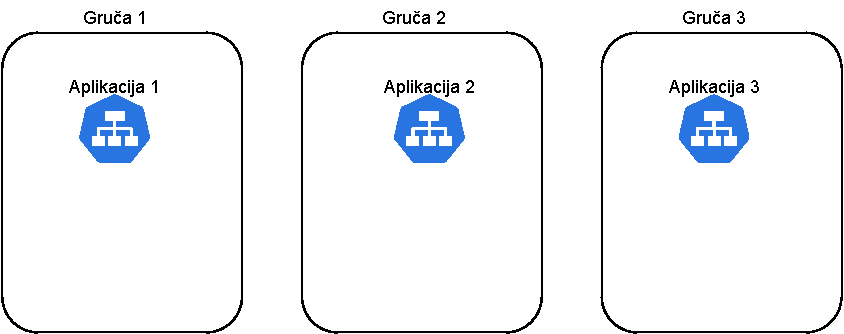
\includegraphics[width=1.0\textwidth]{images/primer-izolirane-aplikacije.pdf}
\end{center}
\caption{Primer izoliranih aplikacij.}
\label{problem-prevelike-latence}
\end{figure}
Ena izmed treh glavnih lastnost federiranih objektov je možnost izbire gruč, na katerih se bo določen objekt ustvaril. 
S tega stališča je naš primer zelo preprost.
Samo določimo, da se naša aplikacija izvaja na gruči 3 namesto na vseh.
Tokrat za federacijo ne moremo uporabiti ukaza \spverb|kubefedctl federate|, ampak moramo spisati konfiguracijo federiranih objektov sami.
Najprej bomo z ukazom \spverb|kubectl tag| označili našo izolirano gručo (ali več njih).
Potem pa bomo lastnosti \spverb|.clusterSelector.matchLabels| vsakega federiranega objekta, ki ga želimo izolirati, dodali označbe vseh izoliranih gruč.
V takšnih primerih se nam ni potrebno posebej ukvarjati s sinhronizacijo podatkov, saj smo ali vse podatke obdržali v isti gruči ali pa sinhroniziramo na enak način kot v poglavju \ref{povezovanje-med-centri}.
\chapter{Upravljanje gruč na robu oblaka}
\label{edge-clusters}
\section{Gruče na robu oblaka}
Razlogov zakaj gruče postavljamo na rob oblaka oziroma fizično bližje konč\-ne\-mu uporabniku je več.
Za primer vzemimo zahtevo podjetja, da se morajo njihovi podatki obdelovati lokalno v njihovem podjetju.
V našem primeru se bomo osredotočali na upravljanje takšnih gruč.
\section{Implementacija s KubeFed}
Ko enkrat povežemo vse gruče z ukazom \spverb|kubefedctl join| je njihovo upravljanje preprosto.
Samo nastavimo v kateri gruči želimo katere objekte in naša naloga je končana.
Zavedati se moramo, da nekaj prenosa podatkov porabi tudi KubeFed za sinhronizacijo, zato moramo biti pozorni, če se podatki prenašajo preko dragih mobilnih omrežji.
\begin{figure}[h]
\begin{center}
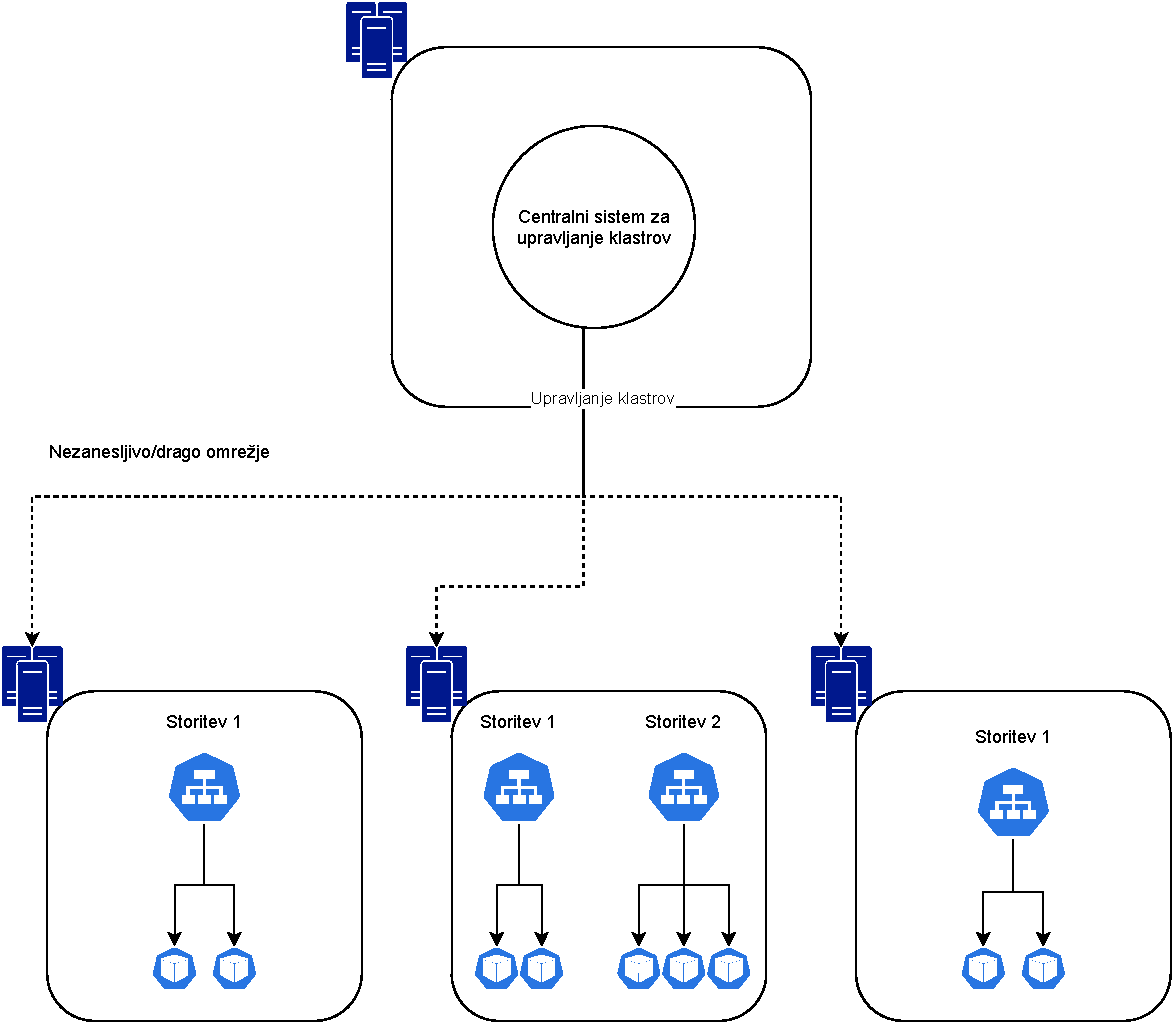
\includegraphics[width=1.0\textwidth]{images/upravljanje-robnih-gruc.pdf}
\end{center}
\caption{Primer upravljanja gruč na robu oblaka.}
\label{problem-prevelike-latence}
\end{figure}

Nam pa KubeFed omogoča še eno možnost s svojo strukturo.
Lahko s svojim kontrolerjem in vmesnikom KubeFed implementiramo še dodatne funkcionalnosti, kot so razporejanje obremenjenosti med lokalnimi strežniki in po potrebi povečujemo število primerkov ali pa kar razporejamo opravila s Kubernetes Job objekti.

Z zelo preprosto integracijo v sistem Kubernetes nam KubeFed vmesnik tu omogoča zelo preprosto implementacijo katerekoli naše rešitve.
\section{Sinhronizacija podatkov}
V primeru gruč na robu oblaka bomo sinhronizacijo verjetno implementirali sami, saj le mi vemo kakšen problem rešujemo in zakaj smo sploh postavljali gruče na robu oblaka.

Za primer vzemimo hipotetični varnostni sistem korporacije, ki centralno spremlja varnost v posameznih podružnicah.
Sistem ima eno nadzorno kamero pri vhodu v vsako podružnico.
Želimo, da naša kamera prepoznava obraze in na podlagi tega dovoljuje zaposlenim vstop.
V našem centralnem sistemu pa želimo, hraniti seznam vstopov.
En način reševanja tega problema je z gručami na robu oblaka.
V vsako podružnico bi postavili gručo rač\-un\-al\-ni\-kov Raspberry PI, ki so dovolj zmogljivi, da obdelujejo posnetke kamer in prepoznavajo obraze.
Če posnetke obdelujemo lokalno, se izognemo pošiljanju veliki količini podatkov na centralne strežnike, posledično pa bo hitrejše tudi preverjanje zaposlenih.
Tako bi na centralni strežnik pošiljali samo številko zaposlenega in čas vstopa.
Takšen pristop bi prišel še toliko bolj do izraza, če imajo podružnice dostop do interneta samo prek dragega mobilnega omrežja, kjer lahko z zmanjšanjem prometa, zelo zmanjšamo tudi stroške podjetja.
Vse te gruče na podružnicah bi imele zelo podobno strukturo in jih je smiselno centralo upravljati s kakšnim sistemom za povezovanje. 
Tu bi lahko uporabili pristop KubeFed ali pristop GitOps.
Pošiljanje podatkov na centrali strežnik pa bi morali napisati sami in ga vgraditi v naš program za prepoznavo obrazov.
\chapter{Sklepne ugotovitve}
V diplomskem delu smo si pogledali teoretično ozadje povezovanja več rač\-un\-al\-ni\-ških gruč in osnove Kubernetesa.
Predstavljenih je bilo tudi nekaj popularnih orodij za delo z več gručami Kubernetes.
V praktičnem delu pa smo se posvetili predvsem reševanju pogostih problemov v industriji, ki zahtevajo povezovanje več gruč.
Zato pa je bilo potrebo postaviti tudi ustrezno okolje za preizkušanje naših rešitev.

Z razvojem Kubernetesa se je razvilo tudi zelo veliko odprtokodnih orodij, ki omogočajo lažje upravljanje in povezovanje več gruč.
Tako so napredne tehnologije prišle v roke širšemu krogu ljudi in jim omogočajo preprostejše reševanje težav.
Kubernetes pa je s standardizacijo orkestracije zelo olajšal tudi možnost gostovanja aplikacije pri več različnih oblačnih ponudnikih, kjer se zopet pojavi problem povezovanja več gruč.

Področje orkestracije in povezovanja gruč se bo še zelo razvijalo in tema bo zagotovo zahtevala še veliko diplomskih del.

\newpage %dodaj po potrebi, da bo številka strani za Literaturo v Kazalu pravilna!
\newpage %dodaj po potrebi, da bo številka strani za Literaturo v Kazalu pravilna!
\newpage %dodaj po potrebi, da bo številka strani za Literaturo v Kazalu pravilna!
\newpage %dodaj po potrebi, da bo številka strani za Literaturo v Kazalu pravilna!
\ \\
\clearpage
\addcontentsline{toc}{chapter}{Literatura}
\bibliographystyle{plain}
\bibliography{literatura}
\end{document}
